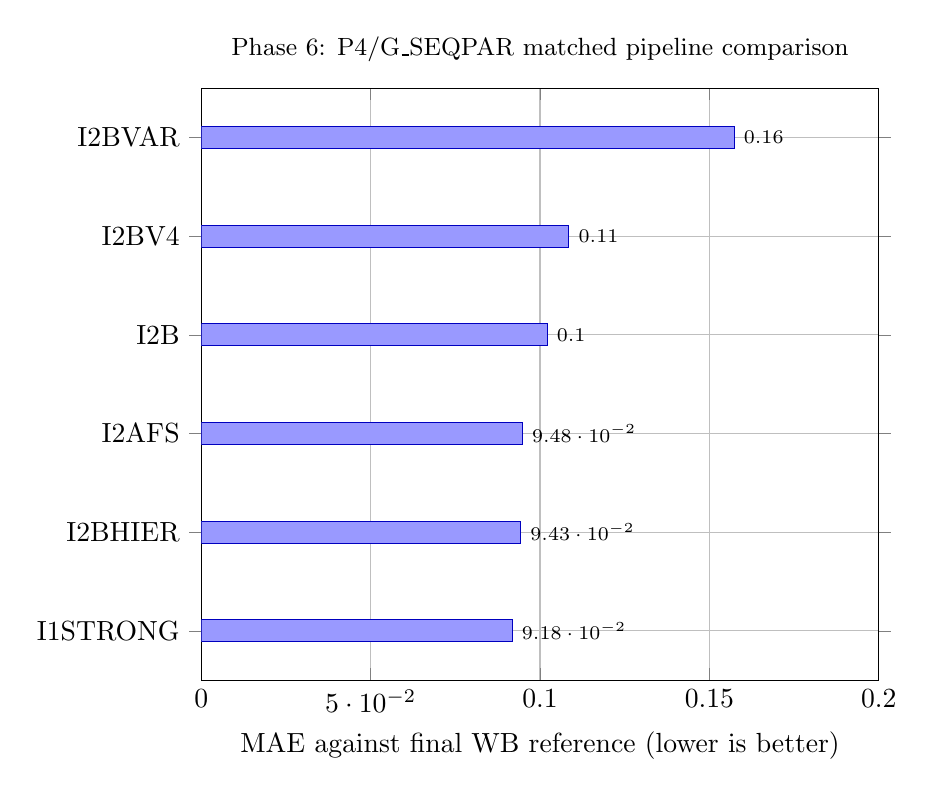
\begin{tikzpicture}
\begin{axis}[
  xbar,width=0.84\linewidth,height=91mm,
  xmin=0,xmax=0.20,xlabel={MAE against final WB reference (lower is better)},
  symbolic y coords={I2BVAR,I2BV4,I2B,I2AFS,I2BHIER,I1STRONG},
  ytick=data,y dir=reverse,
  nodes near coords,nodes near coords align={horizontal},
  every node near coord/.append style={font=\scriptsize},
  xtick={0,0.05,0.10,0.15,0.20},grid=major,
  enlarge y limits=0.10,bar width=8pt,
  title={Phase 6: P4/G\_SEQPAR matched pipeline comparison},
  title style={font=\small}
]
\addplot[fill=blue!40,draw=blue!75!black] coordinates {
(0.091780781,I1STRONG)
(0.094294094,I2BHIER)
(0.094754288,I2AFS)
(0.102096296,I2B)
(0.108538739,I2BV4)
(0.157305372,I2BVAR)
};
\end{axis}
\end{tikzpicture}
